% !TEX root = ../dg.tex

\section{Differential Forms and Vector Calculus}
\label{sec:vector calculus}

Suppose we restrict to the case of a (Riemannian) 3-manifold; that is, a 3-dimensional manifold $M$ endowed with a Riemannian metric $g$ (again, a Riemannian metric is a [smooth] choice of inner product $g_p$ on each tangent space; if this makes you uncomfortable, just assume $M = \R^3$ and we just have the standard dot product on each tangent space). This section is a bit weird and definitely very informal: I'm using a bunch of stuff that I haven't actually defined yet. But the point is to try to say that concepts like \emph{differential forms} and \emph{exterior derivatives} that we will eventually define carefully are just generalizations of things you already understand very well.

From \Crefrange{ex:0-forms and functions}{ex:n-1 forms}, we know that
\[
	\Omega^0(M) = C^\infty(M) \cong \Omega^3(M), \qquad \Omega^1(M) \cong \mathfrak{X}(M) \cong \Omega^2(M), \qquad \text{and} \qquad \Omega^k(M) = \{0\} \text{ for } k > 3.
\]
So anything we can say about differential forms on $M$ must be expressible just in terms of vector fields and functions. We know from vector calculus that there are various differentiation operators on functions and vector fields, namely div, grad, and curl, so what do these mean at the level of forms.

Or, turning it around, are there operations on forms which fill in the squares in the following diagram and makes them commute?

\ifplastex
	\begin{center}
		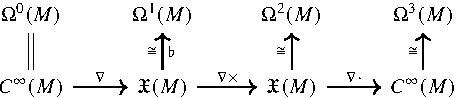
\includegraphics[height=1in]{cd1}
	\end{center}
\else	
	\[
		\begin{tikzcd}
			\Omega^0(M) & \Omega^1(M) & \Omega^2(M) & \Omega^3(M) \\
			C^\infty(M) \arrow[u, equal] \arrow[r,"\nabla"] & \mathfrak{X}(M) \arrow[u,"\cong","\flat"'] \arrow[r,"\nabla\times"] & \mathfrak{X}(M) \arrow[u,"\cong"] \arrow[r,"\nabla \cdot"] & C^\infty(M) \arrow[u,"\cong"]
		\end{tikzcd}
	\]
\fi


First, we (hopefully) recall from vector calculus that the gradient of a function is a vector field, which can be computed in local coordinates as
\[
	\nabla f = \sum_{i=1}^3 \frac{\partial f}{\partial x_i}\frac{\partial}{\partial x_i}.
\]

\begin{exercise}
	If it's not clear, make the effort to connect this to the gradient you're familiar with.
\end{exercise}

Then the corresponding 1-form $(\nabla f)^\flat$ is defined at $p \in M$ by
\[
	(\nabla f)_p^\flat(Y) = g_p(\nabla f, Y) = g_p\left(\sum_{i=1}^3 \frac{\partial f}{\partial x_i} \frac{\partial}{\partial x_i}, \sum_{i=1}^3 b_i(p) \frac{\partial }{\partial x_i}\right) = \sum_{i,j=1}^3 f_{x_i}(p) b_j(p) g_p\left(\frac{\partial }{\partial x_i}, \frac{\partial }{\partial x_j}\right),
\]
where $Y = \sum_{i=1}^3 b_i \frac{\partial }{\partial x_i}$ in local coordinates and I've written $f_{x_i}$ as a shorthand for $\frac{\partial f}{\partial x_i}$.

If we were able to arrange it so that the local coordinate basis $\left\{ \frac{\partial }{\partial x_1},\frac{\partial }{\partial x_2},\frac{\partial }{\partial x_3}\right\}$ were orthonormal with respect to $g_p$, then this would simplify as
\[
	(\nabla f)_p^\flat(Y) = \sum_{i=1}^3 f_{x_i}(p) b_i(p) = \sum_{i=1}^3  b_i(p) \frac{\partial f}{\partial x_i}(p) = \left(\left(\sum_{i=1}^3  b_i \frac{\partial}{\partial x_i}\right)f\right)(p) = (Yf)(p) = df_p(Y)
\]
by \Cref{lem:vector fields and differentials}. In other words, $(\nabla f)^\flat = df$.

Recall (\Cref{ex:1-forms as covectors}) that at each point a 1-form corresponds to a cotangent vector, so the local coordinate basis $\left\{ \frac{\partial }{\partial x_1},\frac{\partial }{\partial x_2},\frac{\partial }{\partial x_3}\right\}$ induces a dual basis which we call $\{dx_1, dx_2, dx_3\}$ for $\left(T_pM\right)^\ast$ defined by 
\[
	dx_i\left(\frac{\partial}{\partial x_j}\right) = \delta_{ij}.
\]
In these terms, 
\[
	df = \frac{\partial f}{\partial x_1} dx_1 + \frac{\partial f}{\partial x_2} dx_2 + \frac{\partial f}{\partial x_3}dx_3.
\]
In other words, in the presence of a Riemannian metric,\footnote{which turns out to be necessary to define the gradient anyway} computing the differential of a function on a 3-manifold (in fact, this works equally well on an $n$-manifold) corresponds to taking the gradient of the function.

Turning to curl, recall that, if $X \in \mathfrak{X}(M)$ is written in local coordinates as $X = a_1 \frac{\partial }{\partial x_1} + a_2 \frac{\partial }{\partial x_2} + a_3 \frac{\partial }{\partial x_3}$, then
\[
	\nabla \times X = \left(\frac{\partial a_3}{\partial x_2} - \frac{\partial a_2}{\partial x_3} \right)\frac{\partial }{\partial x_1} + \left( \frac{\partial a_1}{\partial x_3} - \frac{\partial a_3}{\partial x_1} \right) \frac{\partial }{\partial x_2} + \left( \frac{\partial a_2}{\partial x_1} - \frac{\partial a_1}{\partial x_2} \right) \frac{\partial }{\partial x_3}.
\]

As discussed in \Cref{ex:n-1 forms}, this corresponds to an element of $\omega^{3-1}(M) = \Omega^2(M)$ given by
\[
	\left(\frac{\partial a_3}{\partial x_2} - \frac{\partial a_2}{\partial x_3} \right)dx_2 \wedge dx_3 + \left( \frac{\partial a_1}{\partial x_3} - \frac{\partial a_3}{\partial x_1} \right) dx_3 \wedge dx_1 + \left( \frac{\partial a_2}{\partial x_1} - \frac{\partial a_1}{\partial x_2} \right) dx_1 \wedge dx_2.
\]
For reasons to be explained later, I'm going to call this 2-form $\star (\nabla \times X)^\flat$.

So now what is the operation on $X^\flat = a_1 dx_1 + a_2 dx_2 + a_3 dx_3$ which would have produced $\star (\nabla \times X)^\flat$? The idea is to compute the differential (which is a 1-form) of each coefficient function, and combine it with the corresponding $dx_i$ in a particular way:
\begin{align*}
	d(X^\flat) & = d(a_1 dx_1 + a_2 dx_2 + a_3 dx_3) \\
	& = (da_1) \wedge dx_1 + (da_2) \wedge dx_2 + (da_3) \wedge dx_3 \\
	& = \left( \frac{\partial a_1}{dx_1} dx_1  + \frac{\partial a_1}{dx_2} dx_2 + \frac{\partial a_1}{dx_3} dx_3 \right)\wedge dx_1 + \left( \frac{\partial a_2}{dx_1} dx_1  + \frac{\partial a_2}{dx_2} dx_2 + \frac{\partial a_2}{dx_3} dx_3 \right)\wedge dx_2 \\
	& \qquad \qquad + \left( \frac{\partial a_3}{dx_1} dx_1  + \frac{\partial a_3}{dx_2} dx_2 + \frac{\partial a_3}{dx_3} dx_3 \right)\wedge dx_3 \\
	& = 0 + \frac{\partial a_1}{dx_2} dx_2 \wedge dx_1 + \frac{\partial a_1}{dx_3} dx_3 \wedge dx_1 + \frac{\partial a_2}{dx_1} dx_1 \wedge dx_2 + 0 + \frac{\partial a_2}{dx_3} dx_3 \wedge dx_2 \\
	& \qquad \qquad + \frac{\partial a_3}{dx_1} dx_1 \wedge dx_3 + \frac{\partial a_3}{dx_2} dx_2 \wedge dx_3 + 0 \\
	& = \left(\frac{\partial a_3}{\partial x_2} - \frac{\partial a_2}{\partial x_3} \right)dx_2 \wedge dx_3 + \left( \frac{\partial a_1}{\partial x_3} - \frac{\partial a_3}{\partial x_1} \right) dx_3 \wedge dx_1 + \left( \frac{\partial a_2}{\partial x_1} - \frac{\partial a_1}{\partial x_2} \right) dx_1 \wedge dx_2
\end{align*}
where the rule is that $dx_i \wedge dx_j = - dx_j \wedge dx_i$, which is just the alternating condition on forms. So, if you buy the above manipulations on some level, there is a fairly straightforward generalization of the differential which corresponds exactly to the curl in this setting.

Finally, if $X \in \mathfrak{X}(M)$ is written in local coordinates as $X = a_1 \frac{\partial }{\partial x_1} + a_2 \frac{\partial }{\partial x_2} + a_3 \frac{\partial }{\partial x_3}$, then the divergence is
\[
	\nabla \cdot X = \frac{\partial a_1}{\partial x_1} + \frac{\partial a_2}{\partial x_2} + \frac{\partial a_3}{\partial x_3},
\]
which is a function. But the isomorphism $C^\infty(M) \cong \Omega^3(M)$ described in \Cref{ex:volume form} says that this function corresponds to some 3-form
\[
	\left(\frac{\partial a_1}{\partial x_1} + \frac{\partial a_2}{\partial x_2} + \frac{\partial a_3}{\partial x_3}\right) \dVol_M = \left(\frac{\partial a_1}{\partial x_1} + \frac{\partial a_2}{\partial x_2} + \frac{\partial a_3}{\partial x_3}\right)dx_1 \wedge dx_2 \wedge dx_3
\]
because for an appropriate choice of coordinates I can write $\dVol_M = dx_1 \wedge dx_2 \wedge dx_3$.

Can we get to this 3-form by applying our generalized differential to the 2-form $\star X^\flat = a_1 dx_2 \wedge dx_3 + a_2 dx_3 \wedge dx_1 + a_3 dx_1 \wedge dx_2$? Yes!
\begin{align*}
	d(\star X^\flat) & = d(a_1 dx_2 \wedge dx_3 + a_2 dx_3 \wedge dx_1 + a_3 dx_1 \wedge dx_2) \\
	& = (da_1) \wedge dx_2 \wedge dx_3 + (da_2) \wedge dx_3 \wedge dx_1 + (da_3) \wedge dx_1 \wedge dx_2 \\
	& = \left( \frac{\partial a_1}{dx_1} dx_1  + \frac{\partial a_1}{dx_2} dx_2 + \frac{\partial a_1}{dx_3} dx_3 \right)\wedge dx_2 \wedge dx_3 + \left( \frac{\partial a_2}{dx_1} dx_1  + \frac{\partial a_2}{dx_2} dx_2 + \frac{\partial a_2}{dx_3} dx_3 \right)\wedge dx_3 \wedge dx_1 \\
	& \qquad \qquad + \left( \frac{\partial a_3}{dx_1} dx_1  + \frac{\partial a_3}{dx_2} dx_2 + \frac{\partial a_3}{dx_3} dx_3 \right)\wedge dx_1 \wedge dx_2 \\
	& = \frac{\partial a_1}{dx_1} dx_1\wedge dx_2 \wedge dx_3 + 0 + 0 + 0 + \frac{\partial a_2}{dx_2} dx_2 \wedge dx_3 \wedge dx_1 + 0 + 0 +  \frac{\partial a_3}{dx_3} dx_3 \wedge dx_1 \wedge dx_2 \\
	& = \frac{\partial a_1}{dx_1} dx_1\wedge dx_2 \wedge dx_3 + \frac{\partial a_2}{dx_2} dx_1 \wedge dx_2 \wedge dx_3 + \frac{\partial a_3}{dx_3} dx_1 \wedge dx_2 \wedge dx_3 \\
	& = \left(\frac{\partial a_1}{dx_1} + \frac{\partial a_2}{dx_2} + \frac{\partial a_3}{dx_3}\right) dx_1 \wedge dx_2 \wedge dx_3
\end{align*}

The upshot is that we've now filled in the diagram:

\ifplastex
	\begin{center}
		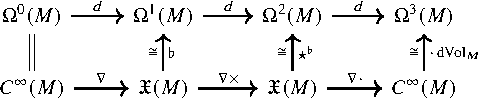
\includegraphics[height=1in]{cd2}
	\end{center}
\else	
	\[
		\begin{tikzcd}
			\Omega^0(M) \arrow[r,"d"] & \Omega^1(M) \arrow[r,"d"] & \Omega^2(M) \arrow[r,"d"] & \Omega^3(M) \\
			C^\infty(M) \arrow[u, equal] \arrow[r,"\nabla"] & \mathfrak{X}(M) \arrow[u,"\cong","\flat"'] \arrow[r,"\nabla\times"] & \mathfrak{X}(M) \arrow[u,"\cong","\star^\flat"'] \arrow[r,"\nabla \cdot"] & C^\infty(M) \arrow[u,"\cong","\cdot \dVol_M"']
		\end{tikzcd}
	\]
\fi


Of course, I haven't really given a rigorous definition of $d$ (which is called the \emph{exterior derivative}), nor of $\wedge$ (the \emph{wedge product}), but, as we will see, there is a natural, coordinate-free way of defining these things for arbitrary differential forms on arbitrary manifolds which specializes to the calculuations above in local coordinates (and hence corresponds to gradient and divergence on manifolds of arbitrary dimension).

Hopefully the fact that div, grad, and curl are all essentially the same operator in this framework helps convince you that differential forms are useful and important. In fact, it gets even better: in this language, the Fundamental Theorem of Calculus, Green's Theorem, and the Divergence Theorem all turn out to be special cases of the same theorem: \emph{Stokes' Theorem for differential forms}.

More than just generalizing essentially all of vector calculus, differential forms also encode topological information (in the form of cohomology). To see this, look again at the diagram above:
\begin{enumerate}
	\item We know from vector calculus that $\nabla \times (\nabla f) = 0$ for any $f \in C^\infty(M)$ and $\nabla \cdot(\nabla \times X) = 0$ for any $X \in \mathfrak{X}(M)$. Since the diagram commutes, this implies that $d \circ d = 0$ regardless of whether you start in $\Omega^0(M)$ or $\Omega^1(M)$ (and in fact this is still true if you start in $\Omega^2(M)$ or $\Omega^3(M)$ since $\Omega^4(M) = \{0\}$). In other words,
	\[
	\ifplastex
		\Omega^0(M) \longrightarrow  \Omega^1(M) \longrightarrow \Omega^2(M) \longrightarrow \Omega^3(M)
	\else
		\begin{tikzcd}
			\Omega^0(M) \arrow[r,"d"] & \Omega^1(M) \arrow[r,"d"] & \Omega^2(M) \arrow[r,"d"] & \Omega^3(M)
		\end{tikzcd}
	\fi
	\]
	is a (co)chain complex. More generally, if we add indices to the exterior derivatives to indicate where they start and end,
	\[
	\ifplastex
		\Omega^0(M) \stackrel{d_0}{\longrightarrow}  \Omega^1(M) \stackrel{d_1}{\longrightarrow}  \dots \stackrel{d_{n-2}}{\longrightarrow} \Omega^{n-1}(M) \stackrel{d_{n-1}}{\longrightarrow} \Omega^n(M) 
	\else
		\begin{tikzcd}
			\Omega^0(M) \arrow[r,"d_0"] & \Omega^1(M) \arrow[r,"d_1"] &  \dots \arrow[r,"d_{n-2}"] & \Omega^{n-1}(M) \arrow[r,"d_{n-1}"] & \Omega^n(M) 
		\end{tikzcd}
	\fi
	\]
	is always a cochain complex on any $n$-manifold (i.e., $d_k \circ d_{k-1} = 0$ for all $k$). The usual thing you do when you have a (co)chain complex is to take the (co)homology, and that's also useful in this case. Doing so yields the \emph{de Rham cohomology groups}
	\[
		H_{\text{dR}}^k(M) := \frac{\ker d_k}{\operatorname{im} d_{k-1}}.
	\]
	In fact, as usual with cohomology, the cohomology groups fit together into a graded ring, and the product operation corresponds to the wedge product $\wedge$. And de Rham cohomology will turn out to be isomorphic to singular (or simplicial) cohomology with real coefficients.
	
	\item In our 3-manifold example, we saw that $\Omega^0(M) = C^\infty(M) \cong \Omega^3(M)$ and $\Omega^1(M) \cong \mathfrak{X}(M) \cong \Omega^2(M)$. In general, if $M$ is an $n$-dimensional manifold, then it will turn out that $\Omega^k(M) \cong \Omega^{n-k}(M)$ for all $k=0, \dots , n$. Even better, this isomorphism descends to the de Rham cohomology groups and we will have that
	\[
		H_{\text{dR}}^k(M) \cong H_{\text{dR}}^{n-k}(M)
	\]
	for all $k$, which is the appropriate version of \emph{Poincaré duality} for de Rham cohomology.
	
\end{enumerate}